\chapter{Supervisor meetings}
The meeting template consist of several parts: place, date and time, when the meeting was organized.
Next, there are lists of presented and absent stakeholders.
After that list of decisions with supporting reason decided on the meeting follows.
Next table summarize action items -- tasks, which must be done and their deadlines.
After that there are listed action items which were finished since last meeting.
Last table summarize pending action items throughout all meetings.
This is followed by summary, which is text description of the meeting and important decisions.
Template is concluded by information about next meeting.

You can see example of single supervisor meeting in next pages.
\label{img:supervisormeeting}

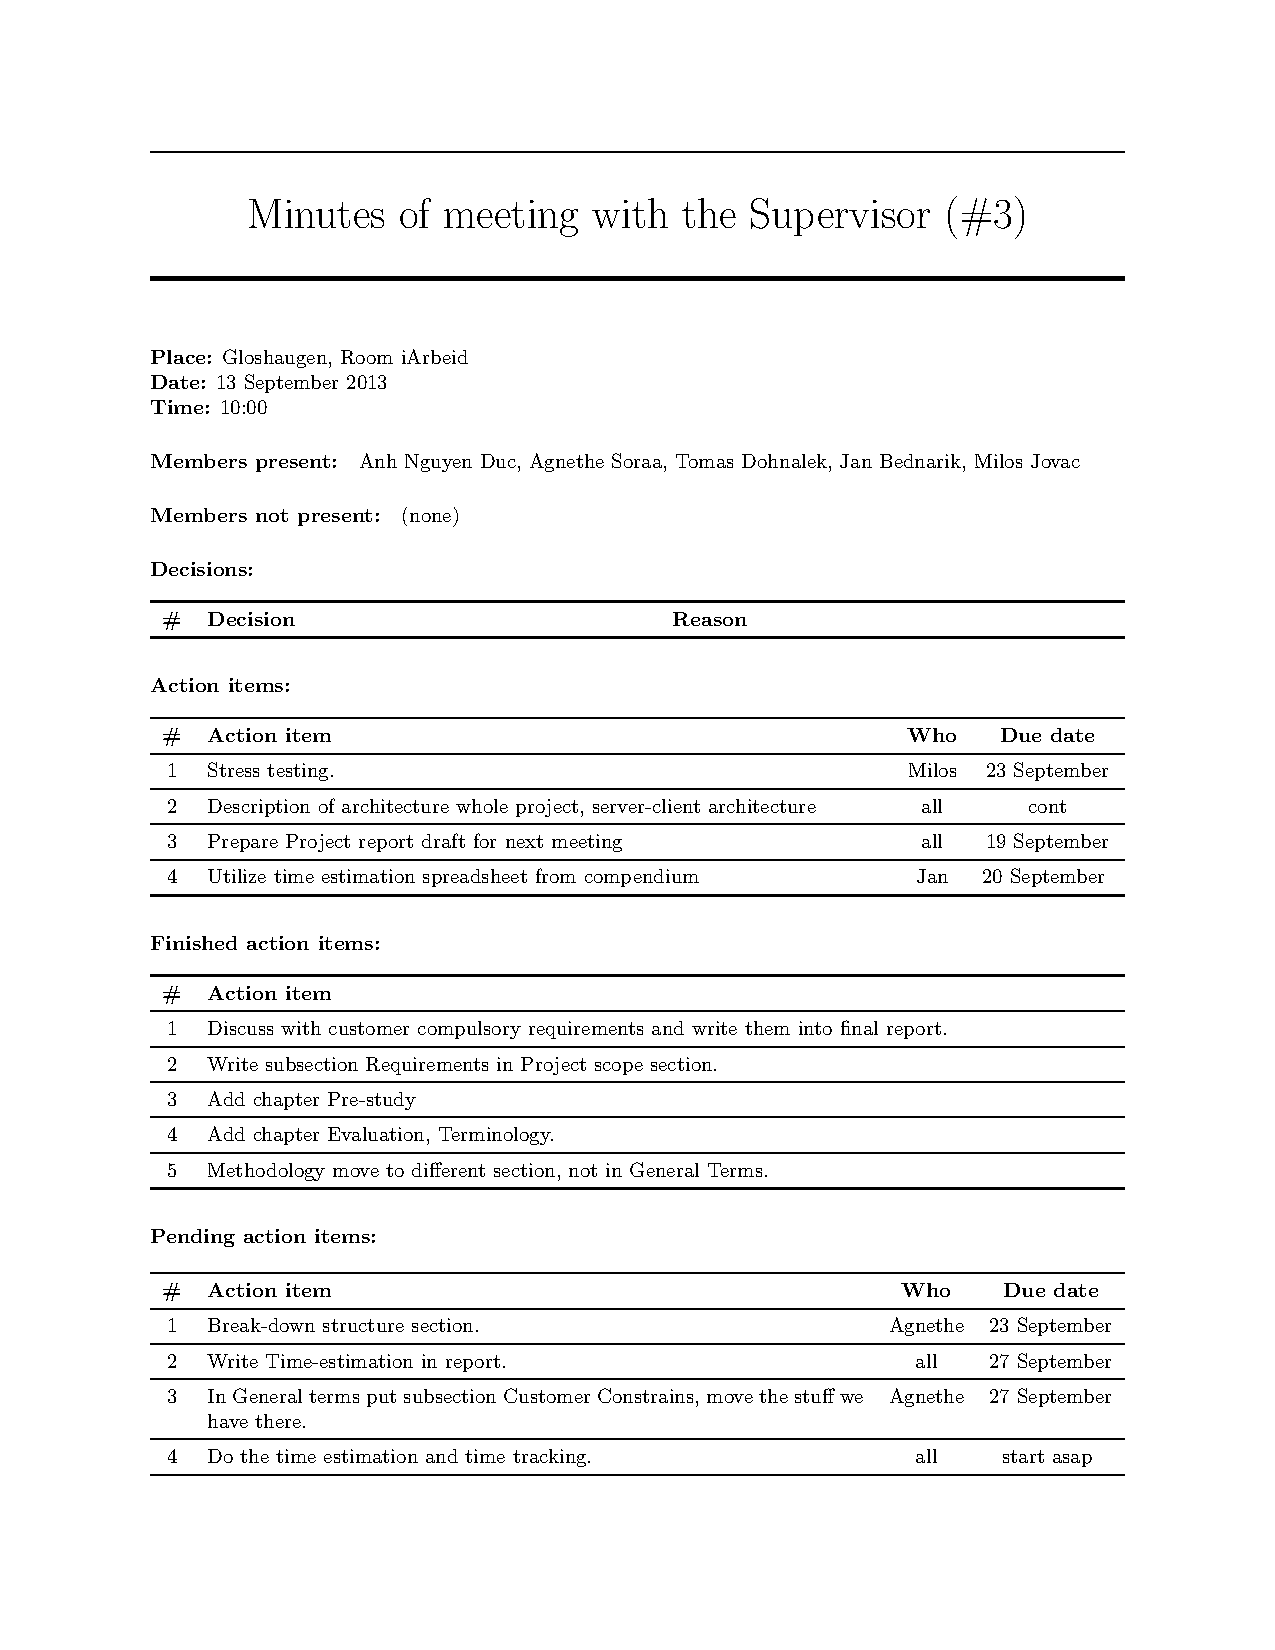
\includepdf[pages=-]{appendix/supervisormeeting.pdf}